\chapter{Modelos y Algoritmos}
\label{chapter:algoritmos}

En esta sección vamos a resolver el problema \problem{Star VRP}, tal como lo definimos en \ref{star-vrp}.

A lo largo de esta sección se intentará ofrecer una notación que sea consistente con la literatura en general, tarea que es por naturaleza irrealizable ya que no hay ningún estándar o convención que lo regule. Lo que sí garantizamos es que va a ser consistente durante todo este escrito.

Si bien fue explicado en detalle en \ref{star-vrp}, por motivos de practicidad a continuación vamos a recordar los parámetros que se utilizarán en todas las secciones de este capítulo. El problema se compone de los siguientes elementos:

\begin{itemize}
    \item Un grafo dirigido y completo $G = (N, E)$.
    \item El conjunto de vehículos disponibles es $K$.
    \item Un conjunto de clientes $S \subseteq N \setminus \{d\}$.
    \item Un nodo distinguido llamado \emph{depósito} y notado $d$, tal que $d \in N$ pero $d \notin S$.
    \item Un valor de \emph{capacidad}, denominada $Q \in \mathbb{Z}^{+}$, que es igual para todos los vehículos.
    \item  $q_s \in \mathbb{Z}^{+}$ la \emph{demanda} asociada al cliente $s$.
    \item Un \emph{conjunto de paradas} $\varrho(s) \subseteq N$ para cada cliente $s$, que es el conjunto de vértices desde las cuales se lo puede atender. Vamos a utilizar como convención que $s \in \varrho(s)$.
    \item El peso de cada arco $(i, j) \in E$ se nota $w_{ij}$.
\end{itemize}

El objetivo del problema es obtener un conjunto de rutas de suma mínima que cumpla las siguientes condiciones:

\begin{itemize}
\label{list:restrictions}
    \item Las rutas son circuitos en el grafo que pasan por el depósito $d$.
    \item Hay a lo sumo tantas rutas como vehículos. Se asigna una ruta a un vehículo (puede haber vehículos sin asignar).
    \item Todos los clientes son atendidos por exactamente un vehículo. Para atender a un cliente $s$, un vehículo debe pasar por alguno de los nodos de $\varrho(s)$.
    \item La suma de las demandas de los clientes atendidos por un vehículo no excede su capacidad.
\end{itemize}

Notemos que se prohíbe que el depósito contenga un cliente, la razón fundamental de esto no es más que practicidad, más adelante queremos evitar que una ruta vacía sea válida, y porque realmente, en términos del lenguaje del problema, no restringe casos interesantes. Esto prueba que $|S| \leq |N|-1$. También utilizamos la convención de que todos los clientes son a su vez paradas (esto es, $s \in \varrho(s)$). 

Ya estamos en condiciones de pasar a la parte más interesante de la tesis, donde se presentan los modelos.


\section{Modelo Compacto}
\label{section:compacto}

El siguiente modelo presenta una cantidad polinomial de variables y restricciones. A los modelos que cumplen esta condición a menudo se los conoce como \emph{modelos compactos} \cite[p.3]{lancia-serafini}.

El modelo intenta encontrar un conjunto de circuitos dirigidos que sean subgrafos de $G$ y que pasen por el depósito. Cada uno de ellos tiene asociado un conjunto de clientes que debe atender y la demanda total de este conjunto no puede superar la capacidad $Q$. La formulación que damos a continuación se basa en esta idea: en cualquier grafo dirigido, un circuito elemental es un subgrafo cuyos vértices tienen todos grado de entrada $d_{in} = 1$ y grado de salida $d_{out} = 1$, y además es fuertemente conexo. Por otro lado, se define \emph{subtour} como un circuito del subgrafo que no pasa por $d$. Para corroborar que este subgrafo sea fuertemente conexo es condición necesaria y suficiente que no existan subtours. En el caso en el que $G$ es un grafo completo, podemos utilizar una serie de restricciones lineales para romper estos subtours, conocidas como \emph{condiciones de Miller-Tucker-Zemlin (MTZ)}.  

\begin{equation}
    \min \sum_{i \in N} \sum_{j \in N} \sum_{k \in K} w_{ij} x_{ijk}
\end{equation}
Sujeto a:
\begin{align}
    \sum_{j \in N, (i, j) \in E}{x_{ijk}} = \sum_{j \in N, (j, i) \in E}{x_{jik}} \qquad & \forall {i \in N, k \in K} \label{eq:compact1} \\
    \sum_{k \in K} y_{sk} = 1 \qquad & \forall {s \in S} \label{eq:compact2} \\
    \sum_{j \in N, (d, j) \in E}{x_{djk}} = 1 \qquad & \forall {k \in K} \label{eq:compact3} \\ 
    y_{sk} \leq \sum_{i \in N}\sum_{v \in \varrho(s)}{x_{ivk}} \qquad & \forall {k \in K, s \in S} \label{eq:compact4} \\
    \sum_{s \in S}{y_{sk}q_s} \le Q \qquad & \forall {k \in K} \label{eq:compact5} \\
u_{ik} - u_{jk} + (|N| - 1)x_{ijk} \leq (|N| - 2)  \qquad & \forall {i \in N, j \in N, k \in K: i,j \neq d, j \neq i} \label{eq:compact6} \\
1 \leq u_{ik} \leq |N| - 1  \qquad & \forall {i \in N, k \in K: i \neq d} \label{eq:compact7} \\
x_{ijk} \in \{0, 1\} \qquad & \forall {i \in N, j \in N, k \in K} \label{eq:compact8} \\
y_{sk} \in \{0, 1\} \qquad & \forall {s \in S, k \in K} \label{eq:compact9}\\
u_{ik} \in \mathbb{Z}^{+} \qquad & \forall {i \in N, k \in K} \label{eq:compact10}
\end{align}

La semántica de las variables es la siguiente: $x_{ijk} = 1$ si y sólo si el vehículo $k$ pasa por el eje $(i, j) \in E$. Por otro lado $y_{sk}$ se interpreta como que el cliente $s$ es atendido por el vehículo $k$. Estas variables \emph{de servicio} se precisan porque el camino de cierto vehículo podría pasar por el cliente pero no atenderlo, por ejemplo, por no tener suficiente capacidad. La clase de variables $u_{ik}$ se utiliza solamente para expresar las condiciones MTZ. 

La ecuación \ref{eq:compact1} garantiza que la cantidad de vehículos que entra al nodo $i$ sea la misma cantidad que sale del nodo $i$. Como explicamos, eso es necesario para que la ruta sea un ciclo. Luego \ref{eq:compact2} asegura que cada cliente es atendido por un y sólo un vehículo. La restricción \ref{eq:compact3} sirve para obligar a cada ruta a pasar por el nodo depósito $d$. La inecuación \ref{eq:compact4} muestra que un cliente $s$ solamente puede ser atendido por el vehículo $k$ si $k$ pasa por alguna parada asociada a $s$, o sea, un nodo $v \in \varrho(s)$. Es importante ver que un vehículo podría visitar a un cliente y sin embargo no atenderlo. La restricción de capacidad se expresa en \ref{eq:compact5}. Por último, \ref{eq:compact6} y \ref{eq:compact7} son las condiciones MTZ para romper subtours.

\section{Generación de Columnas}

En esta sección definimos el modelo extendido sobre el cual aplicaremos un algoritmo de generación de columnas. Para eso comenzamos con una definición que será útil:

\begin{definition}
    (Ruta factible de $G$).
    Llamamos \emph{ruta} de $G$ a un par $r = (C_r, \tilde{S}_r)$ donde $C_r$ es un camino conexo elemental (no repite vértices) de $G$ y $\tilde{S}_r \subseteq S$ un conjunto de clientes. La ruta $r$ se llama \emph{factible} si $C_r$ es un circuito cerrado que pasa por del depósito $d$ y tanto $C_r$ como $\tilde{S}_r$ cumplen las restricciones del problema.
\end{definition}

Tenemos que introducir algunos parámetros que se usarán a continuación. El conjunto $\Omega$ contiene a todas las rutas factibles. Si $r = (C_r, \tilde{S}_r) \in \Omega$, el parámetro $a_{sr} \in \{0, 1\}$ indica si $s \in \tilde{S}_r$, y el parámetro $c_r$ es el costo del circuito $C_r$. 

En la siguiente subsección damos un modelo de programación lineal entera que representa el problema que queremos resolver.

\subsection{Modelo de Set Partitioning}
\label{section:set-partitioning}

\begin{equation}
    \min \sum_{r \in \Omega} c_r  \theta_r
\end{equation}
Sujeto a:
\begin{align}
    \sum_{r \in \Omega} {a_{sr}\theta_r} = 1
\qquad & \forall {s \in S} \label{eq:master1} \\
\sum_{r \in \Omega}{\theta_r} \leq |K| & \label{eq:master2} \\
\theta_r \in \{0, 1\} \qquad & \forall{r \in \Omega}
\end{align}

Las variables binarias $\theta_r$ representan que la ruta $r \in \Omega$ es parte de la solución óptima. Por como definimos $\Omega$, solamente es necesario tomar a lo sumo $|K|$ rutas de este conjunto y asignar una a cada vehículo (pueden quedar vehículos sin utilizar). 

Cada cliente $s$ tiene que ser atendido por un único vehículo, o sea que las rutas deben ser disjuntas en cuanto a los clientes que atienden (no necesariamente en cuanto a los nodos que visitan), y eso se garantiza en \ref{eq:master1}. Finalmente \ref{eq:master2} fuerza que no se elijan más rutas que vehículos disponibles.

\subsection{Restricted Master Problem}
\label{section:rmp}

El lector puede sospechar que si bien el modelo anterior es válido y la solución es exacta, calcular el conjunto $\Omega$ está lejos de ser trivial y aún si nos fuera dado por un oráculo, la cantidad de rutas factibles en él es tal que resultaría, como mínimo, desesperanzador. Llamaremos al modelo de programación lineal de la Sección \ref{section:set-partitioning} el \emph{Problema Maestro}. A continuación se presenta una forma astuta de encararlo.

Sea $\tilde{\Omega} \subset \Omega$ un subconjunto de las rutas factibles  tal que $|\tilde{\Omega}| \ll |\Omega|$. Se define el \emph{Problema Maestro Restringido}, a partir de ahora \problem{RMP}, como un modelo idéntico al problema maestro pero en el cual reemplazamos $\Omega$ por $\tilde{\Omega}$ y así acotamos fuertemente la cantidad de variables $\theta_r$. 

\begin{equation}
    \min \sum_{r \in \tilde{\Omega}} c_r  \theta_r
\end{equation}
Sujeto a:
\begin{align}
    \sum_{r \in \tilde{\Omega}} {a_{sr}\theta_r} = 1
\qquad & \forall {s \in S} \label{eq:rmp1} \\
\sum_{r \in \tilde{\Omega}}{\theta_r} \leq |K| & \label{eq:rmp2} \\
\theta_r \in \{0, 1\} \qquad & \forall{r \in \tilde{\Omega}}
\end{align}

Observemos que la gran mayoría de las rutas de $\Omega$ son rutas \emph{malas}, en el sentido de que son factibles pero no son razonables y no tienen verdaderas chances de ser consideradas como parte de la base. Entonces suena razonable restringir $\tilde{\Omega}$ a un conjunto de rutas \emph{buenas} y resolver un problema más chico, a pesar de que, a priori, podríamos sacrificar la exactitud del problema. El algoritmo de generación de columnas nos permitirá resolver con exactitud la relajación lineal del Problema Maestro resolviendo solamente algunas instancias del Problema Maestro Restringido. Usualmente se complementa esta idea con un algoritmo de Branch \& Price, si estamos interesados en encontrar el óptimo exacto (es decir, el óptimo del problema maestro con restricciones de integralidad y no de la relajación lineal), lo cual queda vacante en esta tesis.	

En cada iteración del algoritmo Simplex existe una fase donde se evalúan los costos reducidos de todas las variables y se elige el menor para insertar esa variable en la base. Cada costo reducido se calcula como $\bar{c}_r = c_r - \lambda^{T}a_r$ donde $\lambda$ es el vector de variables duales y $a_r$ es la columna de coeficientes asociados a la variable $r$. Se puede demostrar que introducir en la base la variable $\theta_r$ de costo reducido negativo garantiza que en la próxima iteración de Simplex se obtendrá una solución mejor, y más aún, que si no existen costos reducidos negativos, el problema está resuelto a optimalidad. Supongamos que resolvimos el \problem{RMP}, cuya solución trivialmente también es factible en el problema maestro. Si algún costo reducido es negativo, podemos agregar esta variable a $\tilde{\Omega}$ y lo volvemos a resolver; si no existen tales, ya habremos encontrado el óptimo del Problema Maestro. El proceso de encontrar nuevas variables para agregar a $\tilde{\Omega}$ e iterar hasta que no queden más es lo que se conoce como \emph{Generación de Columnas}.

El problema aún persiste, porque calcular \emph{todos} los costos reducidos explícitamente implica hacer una operación por cada variable de $\Omega$, y eso es inaceptable. Necesitamos conseguir una manera eficiente de saber cuál es el menor $\bar{c}_r$ sin tener que calcularlos todos explícitamente. Este problema se conoce como \emph{subproblema de pricing}. La fortaleza de generación de columnas por lo general subyace en que exista una formulación eficiente para resolver el pricing.

\begin{algorithm}[H]
    \caption{Algoritmo de generación de columnas}
    \label{al:column-generation}
    \begin{algorithmic}[1]
        \Require El problema maestro. 
        \Ensure El óptimo $\Theta^{*}$ de la relajación lineal del problema maestro. 
        \State Sea $\Theta = \{\theta_1 = 1, \dots, \theta_k = 1\}$ una solución factible inicial
        \If{$\Theta = \emptyset$}
            \Return Problema infactible
        \EndIf
        \State $\tilde{\Omega} \gets \Theta$
        \While{ \textbf{true} }
            \State Resolver RMP y su dual, restringidos a $\tilde{\Omega}$
            \State Sea $\Theta^{*}$ el óptimo del RMP.
            \State Sea $\lambda$ el vector de variables duales.
            \State Resolver subproblema de pricing.
            \State $r^{*} \gets \argmin_{r \in \Omega}{\bar{c}_r}$ // $r^{*}$ es la ruta con menor costo reducido
            \If{$\bar{c}_{r^{*}} \geq 0$}
            	\Break
            \EndIf
            \State $\tilde{\Omega} \gets \tilde{\Omega} \cup \{\theta_{r^{*}}\}$
        \EndWhile
        \Return $\Theta^{*}$
    \end{algorithmic}
\end{algorithm}

El Algoritmo \ref{al:column-generation} requiere que comencemos resolviendo el \problem{RMP} con un $\tilde{\Omega}$ válido, para luego calcular las variables duales que necesita el problema de pricing. No existe hasta donde sabemos una manera mecánica de elegir este conjunto. Para que el problema restringido resulte al menos factible, se precisa una heurística que provea una solución factible inicial. No es crítico en este paso que la solución esté demasiado cerca del óptimo, por lo que se priorizarán heurísticas rápidas. Proveemos una heurística en la Sección \ref{section:initial-solution-heuristic}, sin embargo, ésta podría reportar que no existen soluciones factibles cuando sí las hay, y en ese caso en \ref{feasibility-problem} damos un algoritmo infalible aunque mucho más lento.

Desrochers et al. discuten en \cite{desrochers1992} si conviene modificar levemente el \problem{RMP} para aliviar la fase de pricing. La igualdad en \ref{eq:rmp1} se reemplaza por una desigualdad que no descarta soluciones factibles pero que resulta computacionalmente menos costosa:

\begin{equation}
\label{eq:ge-restriction-rmp}
     \sum_{r \in \tilde{\Omega}} {a_{sr}\theta_r} \geq 1
\qquad \forall {s \in S}
\end{equation}

Esto se interpreta como que cada cliente debe ser atendido por uno o más vehículos. Notemos que una solución factible de este problema modificado que no es factible en el original solamente tiene clientes repetidos (atendidos por múltiples vehículos), lo cual no cambia el valor de la función objetivo.

En el ejemplo de \cite{desrochers1992} la ganancia es clave: el problema de pricing ahora no requiere que los caminos sean elementales y la solución sigue siendo factible. En nuestro caso tenemos una complicación extra, porque la nueva formulación admite clientes repetidos y eso contradice una condición del problema, entonces surge la necesidad de agregar una fase de post-procesamiento de la solución, para eliminarlos.


\subsection{Problema dual}

Será útil calcular el problema dual de la relajación lineal del Restricted Master Problem. Esto nos servirá más adelante para calcular los costos reducidos de las variables del RMP. 
Dado que éste tiene $|S| + 1$ desigualdades, en el dual hay $|S| + 1$ variables, que las llamaremos $\lambda_s$ para $s \in \{0, \dots, |S|\}$. Utilizamos la siguiente convención: $\lambda_0$ es la variable dual asociada a \ref{eq:rmp2} y $\lambda_{s}$ es la variable asociada al $s-$ésimo cliente de $S$ de \ref{eq:rmp1}.
\\

\begin{equation}
    \max \sum_{s \in S} \lambda_s + |K| \lambda_0 
\end{equation}

Sujeto a:

\begin{align}
    \lambda_0 + \sum_{s \in S} {a_{sr} \lambda_s} \leq c_r \qquad & \forall {r \in \Omega} \\
\lambda_s \in \mathbb{R} \quad \text{libre}
\qquad &\forall {s \in S} \\
\lambda_0 \geq 0 &
\end{align}

Cabe aclarar que si en el RMP se utiliza la desigualdad \ref{eq:ge-restriction-rmp} en lugar de la igualdad \ref{eq:rmp1}, el problema dual permanece igual salvo por que la clase de variables $\lambda_s$ cambia su rango a $\lambda_s \leq 0$. 


\subsection{Heurística para una solución inicial}
\label{section:initial-solution-heuristic}

El algoritmo de generación de columnas necesita que en cada iteración tengamos una solución factible del problema maestro, incluida la primera, que luego es utilizada por el subproblema de pricing. Por eso desarrollamos una heurística que encuentra una asignación de rutas factible para \problem{Star VRP}.

Esta heurística depende fuertemente del hecho de que $G$ es completo. Vamos a empezar con una definición.

\begin{definition}
    (Partición factible de clientes).
    Una partición de $S$ en $n$ subconjuntos $\{S_1, \dots, S_n\}$ se llama \emph{factible} si estos son disjuntos dos a dos, su unión es $S$, y se cumple que $\sum_{s \in S_i} q_s \leq Q$ para todo $1 \leq i \leq n$, es decir, que la suma de las demandas en cada subconjunto no supera la capacidad.
\end{definition}

Como el grafo es completo, siempre existe un circuito que parte del depósito, recorre todos los vértices de $S_i$ en algún orden y vuelve al depósito. Esto ya nos da una idea de cómo va a ser el algoritmo, aunque nos falta ver algo más. 

\begin{definition}
    (Partición minimal y mínima de clientes).
    Una partición factible de $S$ se dice \emph{minimal} si no existen dos subconjuntos $S_i, S_j$ tales que $\sum_{s \in S_i \cup S_j} q_s \leq Q$. Se dice que esta partición es \emph{mínima} si no existe una partición minimal de cardinal menor.
\end{definition}

Si tenemos una partición factible de clientes de tamaño $n$ y se cumple que $n \leq |K|$, el problema quedaría resuelto, ya que vimos cómo construir una ruta para cada uno de estos conjuntos. Primero veremos una heurística eficiente para encontrar esta partición. El caso en el que $n > |K|$ es difícil de tratar y será estudiado más adelante. Observemos además que si el problema no es factible, no existe tal partición de clientes.

\begin{observation}
    \label{obs:heuristic-observation}
    \problem{Star VRP} es factible si y sólo si existe una partición factible mínima de clientes de tamaño a lo sumo $|K|$.
\end{observation}

Proponemos dividir la heurística en dos partes: un algoritmo que construye una partición factible minimal y otro que crea los circuitos a partir de la partición.

\begin{algorithm}[H]
  \caption{Algoritmo para construir una partición factible minimal}
  \label{al:feasible_minimal_partition_algorithm}
  \begin{algorithmic}[1]
  	\Require $S$ un conjunto de clientes.
  	\Ensure Una partición factible minimal $\mathscr{P}$.
        \State $\text{demanda} \gets 0$
        \State $i \gets 0$
        \ForEach {$s \in S$}
            \State $\text{demanda} \gets \text{demanda} + q_s$
            \If {$\text{demanda} > Q$}
                \State $i \gets i + 1$
                \State $\text{demanda} \gets q_s$
            \EndIf
            \State $S_i = S_i \cup \{s_i\}$
        \EndFor
        \State $n \gets i$
	\Return $\mathscr{P} = \{S_1, \dots, S_n\}$
  \end{algorithmic}
\end{algorithm}

El primer algoritmo nos garantiza encontrar una solución minimal, aunque no necesariamente mínima. El segundo algoritmo es heurístico y da como resultado la solución factible que necesitamos. Toma como parámetro el resultado del algoritmo anterior. Es importante notar que si $n > |K|$ no podemos utilizarlo, y tenemos que proceder como se explica en \ref{feasibility-problem}.

\begin{algorithm}[H]
  \caption{Heurística para construir una solución factible.}
  \label{al:feasible_solution_heuristic}
  \begin{algorithmic}[1]
  	\Require $\mathscr{P}$ una partición factible minimal de clientes.
  	\Ensure Un conjunto de rutas que cumple las restricciones de \problem{Star VRP}.
        \ForEach{$S_i \in \mathscr{P}$}
            \State $\text{ruta}_i \gets \emptyset$
            \State $\text{AgregarNodo(ruta}_i \text{, } d \text{)}$
            \ForEach{$v \in S_i$}
                \State $\text{AgregarNodo(ruta}_i \text{, } v \text{)}$
            \EndFor
            \State $\text{AgregarNodo(ruta}_i \text{, } d \text{)}$
        \EndFor
	\Return $\{\text{ruta}_1, \dots, \text{ruta}_n\}$
  \end{algorithmic}
\end{algorithm}

En este problema se tomó la decisión de que no es necesario utilizar los $|K|$ vehículos. Sin embargo, si este no fuera el caso, el algoritmo se puede adaptar fácilmente: si $n = |K|$, no hay nada que hacer, y si $n < |K|$, entonces tenemos que romper la condición de minimalidad. Basta con tomar un subconjunto cualquiera $S_i \in \mathscr{P}$ y hacerlo atravesar una suerte de mitosis que haga resultar dos conjuntos en lugar de uno. Llamemos $\mathscr{P'}$ a la nueva partición, entonces queda $S_i = S_i \setminus \{s\}$ y se crea un nuevo conjunto $S_{n+1} = \{s\}$, de manera que $|\mathscr{P'}| = |\mathscr{P}| + 1$. Realizamos este proceso hasta que la partición resultante tenga el tamaño buscado.

Es importante aclarar que esta heurística puede no encontrar soluciones factibles en caso de haberlas, y si esto llegase a ocurrir estamos obligados a correr otro algoritmo que resuelve este problema, que se detalla en la próxima sección.


\subsubsection{Problema de factibilidad}
\label{feasibility-problem}

En la práctica raramente la heurística no encuentra una solución factible en caso de haberla. Pero si éste es el caso, existe una manera de sortear esta dificultad. Para esto proponemos el siguiente algoritmo.

Supongamos que el Algoritmo \ref{al:feasible_minimal_partition_algorithm} arroja una partición minimal que no es mínima, y que con mucha mala suerte, la partición tiene mayor al tamaño de la flota de vehículos ($n > |K|$) pero el problema sí es factible: por la Observación \ref{obs:heuristic-observation} debe existir una partición que tenga tamaño menor o igual que $|K|$. Para resolver esto daremos un modelo de programación lineal entera. Una observación clave es la siguiente: este modelo es factible si y sólo si el problema original es factible, por lo tanto, sería justo que llamemos al problema de encontrar la partición mínima como \emph{problema de factibilidad}. Dado que solamente queremos determinar la existencia de una solución, no es un problema de optimización y se puede prescindir de la función objetivo:

\begin{align}
    \sum_{s \in S}{\omega_{sk} q_s} \leq Q \qquad & \forall {k \in K} \label{eq:feasibility1} \\
    \sum_{k \in K}{\omega_{sk}} = 1 \qquad & \forall {s \in S} \label{eq:feasibility2} \\
    \omega_{sk} \in \{0, 1\} \qquad & \forall {s \in S, k \in K} \label{eq:feasibility3}
\end{align}

La variable $\omega_{sk}$ vale $1$ si el $k-$ésimo subconjunto contiene al cliente $s$, caso contrario vale $0$. Basta con encontrar una asignación para la clase de variables $\omega_{sk}$ para resolver el problema, y por lo tanto la función objetivo se puede ignorar. 

La restricción en \ref{eq:feasibility1} indica que la demanda de los clientes atendidos por un vehículo no pueden superar la capacidad del mismo y la ecuación \ref{eq:feasibility2} prohíbe que un cliente sea atendido por más de un vehículo. 

El problema de asignar $|S|$ elementos distintos en $|K|$ conjuntos de suma acotada aparece en muchos ámbitos de la investigación operativa. Por ejemplo, se puede pensar en términos del \problem{Bin Packing Problem} en su versión de decisión: si tenemos $|K|$ cajas de capacidad fija $Q$ en las cuales deben ordenarse $|S|$ elementos, cada uno de ellos de tamaño $q_s$, entonces ambos problemas son equivalentes. Esto nos hace sospechar que no existen algoritmos eficientes que resuelvan de manera exacta el problema de factibilidad, dado que el \problem{Bin Packing Problem} de decisión es NP-Completo. 

El Algoritmo \ref{al:column-generation} requiere que siempre exista una solución factible inicial, entonces si la heurística de la Sección \ref{section:initial-solution-heuristic} falla (no encuentra ninguna solución factible), nos vemos obligados a encontrarla corriendo el modelo que acabamos de describir, lo cual no sería deseable por razones relacionadas a su eficiencia computacional.


\subsection{Subproblema de Pricing}

Resolver el subproblema de pricing es equivalente a encontrar una columna del \problem{RMP} en \ref{section:rmp} que tenga costo reducido negativo.

En primera instancia, estamos resolviendo la relajación lineal de \ref{section:rmp}, y por eso podemos usar las variables de su problema dual. Sea $\{\lambda^*_0, \dots, \lambda^*_{|S|}\}$ la solución óptima del dual. 
El costo reducido de la variable $\theta_r$ se calcula de la siguiente manera:

\begin{equation}
    \bar{c}_r = c_r - \lambda^*_0 - \sum_{s \in S}{a_{sr}\lambda^*_s} 
\end{equation}

Ahora estamos intentando encontrar una ruta $r \notin \tilde{\Omega}$, cuyo costo es $c_r$ y que visita a los clientes $\tilde{S}_r = \{s_0, \dots, s_i\} \subseteq S$, de manera que $\bar{c}_r = c_r - \lambda^*_0 - \sum_{s \in \tilde{S}_r}{\lambda^*_s} < 0$. Para esto es útil la siguiente definición:

\begin{definition}
    (Precio de una ruta factible).
    El precio de una ruta factible se calcula como: 
    \begin{equation}
        \bar{c}_r = \sum_{(i, j) \in E}{w_{ij}} - \lambda^*_0 - \sum_{s \in \tilde{S}_r}{\lambda^*_s}
    \end{equation}
\end{definition}

La semántica del problema de pricing ahora se transforma en querer encontrar una ruta factible sobre $G$ cuyo precio sea menor a $0$. Estamos en condiciones de dar una definición formal del problema que vamos a resolver. 

\optpr{Star ESPPRC}{
Un grafo $G=(N, E)$, el depósito $d$ y las variables duales $\{\lambda^*_0, \dots, \lambda^*_{|S|}\}$
}{
La ruta factible de $G$ de menor precio.
}
\label{star-pricing}

Esto indica que puede ser razonable pensar \problem{Star ESPPRC} como un problema de caminos mínimos sobre grafos. La sigla en cuestión hace referencia al problema del camino mínimo elemental con restricciones de recursos (en inglés: Elementary Shortest Path Problem with Resource Constraints). Se discute en profundidad este problema y su relación con \problem{Star Routing} en \ref{section:espprc}.


\section{Algoritmos de Pricing}
\label{section:pricing-algorithms}

En esta sección presentamos algunos algoritmos que resuelven \problem{Star ESPPRC} de manera exacta y otros que lo resuelven de manera aproximada pero mucho más eficientemente. Como el subproblema de pricing se transformó en un problema de caminos mínimos, antes de proceder a explicar cómo resolverlo es necesario entender cómo se modela el grafo y definir algunos parámetros.


\subsection{ESPPRC}
\label{section:espprc}

El subproblema de pricing en una gran cantidad de variantes de \problem{VRP} es modelado por muchos autores como el problema del camino mínimo elemental con restricciones de recursos (\problem{ESPPRC} de ahora en más). Vamos a tomar la definición que dan Poggi \& Uchoa en \cite{poggi-uchoa}. 

El problema se define sobre un grafo dirigido $G = (N \cup \{n+1\}, E)$, donde el vértice $n+1$ es una copia del depósito y $E$ es el conjunto completo de arcos quitando las aristas salientes del vértice $n+1$ y las aristas entrantes al depósito. En otras palabras, el depósito actúa como nodo fuente, que llamaremos $v_s$, y el nuevo nodo $n+1$ es un sumidero, a partir de ahora $v_e$. Por cada arista $(i, j) \in E$, existe un costo $w_{ij}$, no necesariamente positivo. Se define un conjunto $H$ de \emph{recursos}. Cada recurso $h \in H$ tiene una disponibilidad $C_h \in \mathbb{Z}^{+}$ y por cada arco $(i, j) \in E$ existe una cantidad entera $d_{ij}^{h}$ llamada \emph{consumo} del recurso $h$. El problema \problem{ESPPRC} tiene el objetivo de hallar el camino mínimo elemental que comience en $v_s$ y termine en $v_e$ tal que por cada recurso $h \in H$ el consumo total $T_h$ no supere la capacidad $C_h$. 

Una aclaración importante es que para problemas de camino mínimo es usual que para los nodos fuente y sumidero se empleen los nombres $v_s$ y $v_e$, que en el caso del depósito difiere de la notación de las secciones anteriores (antes lo llamábamos $d$), por lo tanto, en esta subsección y en las que vemos cómo resolver \problem{ESPPRC} utilizando algoritmos sobre grafos (Secciones \ref{section:pricing-pulses} y \ref{section:pricing-labeling}), el lector puede esperar que utilicemos estos nuevos nombres.

Ahora, veamos que podemos expresar el problema de pricing de \problem{Star VRP} detallado en \ref{star-pricing} en términos de un \problem{ESPPRC} levemente modificado. La principal diferencia es que en nuestro modelo, el consumo de recursos no se efectúa al recorrer una arista sino o bien al atravesar un vértice, o bien al atender a un cliente. Existe un único recurso, $1$, tal que $C_1 = Q$ y $d_{s}^{1} = q_s$. Además, cada vez que se decide atender un cliente $s$ el precio acumulado disminuye en una cantidad igual a $\lambda^{*}_s$.

Siguiendo la idea de que cada cliente $s$ tiene asociado un conjunto de paradas $\varrho(s) \subseteq N$, ahora sería útil definir el concepto inverso, o sea, el conjunto de clientes asociados a una parada en un vértice $v$.

\begin{definition}
    (Conjunto de clientes asociados a una parada).
    Se dice que el cliente $s \in S$ está asociado a la parada $v \in N$ si $v$ es una parada que puede atender a $s$, esto es, si $v \in \varrho(s)$. El conjunto de todos los clientes asociados a $v$ se denota $\varrho^{-1}(v) \subseteq S$.
\end{definition}

\subsection{Modelo de Pricing usando PLE}
\label{section:pricing-ple}

El enfoque estándar para resolver este problema es crear un modelo de programación lineal entera que resulta ser muy similar al modelo compacto de la Sección \ref{section:compacto}. Se pueden pensar las restricciones de este modelo como el equivalente \emph{monovehículo} del modelo compacto, aunque la función objetivo difiere. 

\begin{equation}
\min \sum_{(i, j) \in E} {x_{ij} w_{ij}} - \sum_{s \in S} {y_{s} \lambda^*_s - \lambda^*_0}
\end{equation}

Sujeto a:

\begin{align}
    \sum_{j \in N, (i, j) \in E}{x_{ij}} = \sum_{j \in N, (j, i) \in E}{x_{ji}} \qquad & \forall {i \in N} \label{eq:pricing1} \\
    \sum_{j \in N, (d, j) \in E}{x_{dj}} = 1 & \label{eq:pricing2} \\
    y_{s} \leq \sum_{i \in N}\sum_{v \in \varrho(s)}{x_{iv}} \qquad & \forall {s \in S} \label{eq:pricing3} \\
    \sum_{s \in S}{y_{s}q_s} \le Q & \label{eq:pricing4} \\
    u_{i} - u_{j} + (|N| - 1)x_{ij} \leq (|N| - 2) \qquad & \forall {i \in N, j \in N : i, j \neq d, j \neq i}  \label{eq:pricing5} \\
    1 \leq u_{i} \leq |N| - 1 \qquad & \forall {i \in N : i \neq d} \label{eq:pricing6} \\
    x_{ij} \in \{0, 1\} \qquad & \forall {i \in N, j \in N} \label{eq:pricing7} \\
y_{s} \in \{0, 1\} \qquad & \forall {s \in S} \label{eq:pricing8}\\
u_{i} \in \mathbb{Z}^{+} \qquad & \forall {i \in N} \label{eq:pricing9}
\end{align}

Se ve que las variables del modelo son similares a las que explicamos en \ref{section:compacto}. La clase de variables $x_{ij}$ demarcan que el circuito utiliza el arco que une el nodo $i$ con el nodo $j$. Las variables $y_s$ son positivas si y sólo si la ruta visita y atiende al cliente $s$. Por último tenemos las variables $u_i$ que son la forma clásica de escribir las condiciones MTZ.

La ecuación \ref{eq:pricing1} indica que la cantidad de arcos que entra al nodo $i$ tiene que ser igual a la cantidad de arcos que salen, para cumplir con la condición de circuito. Además, \ref{eq:pricing2} especifica que el camino tiene que pasar por el depósito. La restricción \ref{eq:pricing3} se interpreta como que un cliente solamente puede ser atendido por un vehículo que pasa por una parada asociada válida. La restricción de capacidad se expresa en \ref{eq:pricing4} y finalmente las restricciones \ref{eq:pricing5} y \ref{eq:pricing6} son las condiciones MTZ para romper subtours y asegurar que el recorrido sea conexo.

\subsection{Modelo de Pricing con un algoritmo de pulsos}
\label{section:pricing-pulses}

Discutimos en la Sección \ref{section:rmp} que la fortaleza de los algoritmos de generación de columnas por lo general recae en encontrar una formulación eficiente para el problema de pricing. La buena noticia es que como el marco de trabajo es suficientemente flexible, entonces no estamos obligados a resolver este problema de optimización con programación lineal entera. A continuación se detalla un algoritmo sobre grafos, que es a resumidas cuentas un backtracking que utiliza búsqueda en profundidad (DFS), con varias podas eficientes. El trabajo está fuertemente basado en una publicación de Lozano, Duque \& Medaglia \cite{lozano-duque-medaglia} que fue particularmente relevante ya que proponen un algoritmo innovador para resolver \problem{ESPPRC}. Si bien la publicación originalmente se enfoca a instancias de \problem{VRPTW}, no resultará difícil encontrar un algoritmo para \problem{Star VRP}.

Vamos a utilizar la analogía de un \emph{pulso} se propaga a través de un grafo. La \emph{propagación} comienza en el nodo inicial a todos sus vecinos, que a su vez pueden o bien extenderlo recursivamente, hasta llegar al nodo final, o bien descartarlo si alguna de las restricciones de recursos es violada. El pulso de menor precio que llega hasta el nodo destino sería la solución al problema. Notemos que es un algoritmo exacto y que siempre termina si no se permite que el pulso revisite vértices, ya que la cantidad de caminos elementales del inicio al final es finita y se los recorre todos. 

\subsubsection{Representación y variables del problema}

El \emph{pulso} se define como una señal que comienza en el vértice $v_s$ y debe recorrer todas las combinaciones posibles de caminos que llegan hasta el destino $v_e$ y de clientes que potencialmente puede atender. Llamamos \emph{camino parcial} a la trayectoria que realizó el pulso hasta llegar a la posición actual. Un camino parcial $C$ tiene las siguientes propiedades:

\begin{itemize}
    \item $r(C)$ es el precio acumulado de $C$, es decir, el costo del camino menos un valor $\lambda^{*}_s$ descontado por cada cliente visitado.
    \item $q(C)$ se refiere a la demanda acumulada por los clientes visitados.
    \item $p(C)$ es una lista de los vértices que visitó $C$
    \item $s(C)$ es el conjunto de clientes atendidos.
\end{itemize}

Notemos que en este nuevo lenguaje el problema se transforma en encontrar el camino parcial que llega a $v_e$ y tiene menor $r(C)$ satisfaciendo $q(C) \leq Q$.


\subsubsection{Algoritmo de pulsos}

El algoritmo necesita dos reglas de propagación, para visitar todas las combinaciones de nodos y clientes. En cada paso el pulso tiene dos opciones, o bien reproducirse y propagarse a todos los vecinos del vértice actual, transmitiendo a cada uno de sus descendientes la información que recolectó en su duración de vida, o bien sumar un cliente válido al acumulado. La primera regla se llama regla de \emph{propagación a nodos} y la segunda de \emph{propagación a clientes}. Ahora bien, surge la necesidad de definir una función que en cada paso valide si el pulso es \emph{factible}, y que además tenga la capacidad de descartar pulsos subóptimos. Para el descarte se utilizarán dos heurísticas. La primera utiliza una matriz de tamaño $|N| \times (Q+1)$ que contiene cotas inferiores para el precio restante hasta que el pulso llegue a destino. La segunda heurística tiene la capacidad de deshacer las últimas elecciones de propagación en caso de que se tenga alguna certeza de que nos dirigimos a una sección del espacio de búsqueda poco prometedora.

El algoritmo se divide en tres partes. La primera rutina es el algoritmo maestro que solamente inicia la propagación y también llama al esquema de acotaciones que calcula la matriz de costos inferiores. La segunda parte se encarga de propagar recursivamente los pulsos hasta llegar al destino, o bien de descartarlos. Existen tres reglas de descarte que serán explicadas más adelante. Por último aparece el algoritmo que precalcula las cotas inferiores.

\begin{algorithm}[H]
  \caption{Algoritmo maestro}
  \label{al:pulse-master}
  \begin{algorithmic}[1]
  	\Require Un grafo $G = (N, E)$ y las variables duales $\{\lambda^*_0, \dots, \lambda^*_{|S|}\}$.
  	\Ensure La ruta factible de menor precio $\mathscr{R}^{*}$.
        \State $\texttt{bound()}$
        \State $\texttt{pulse(} d, \emptyset \texttt{)}$
	\Return $\mathscr{R}^{*}$
  \end{algorithmic}
\end{algorithm}

El proceso \texttt{bound} se detalla en el Algoritmo \ref{al:pulse-bound}, que es donde se construye la matriz de cotas inferiores. El procedimiento \texttt{pulse} (Algoritmo \ref{al:pulse-node-propagation}) comienza a propagar el pulso, inicialmente con la regla \emph{propagación a nodos}. El valor $\mathscr{R}^{*}$ funciona como una variable global que indica la mejor ruta encontrada hasta el momento y se actualiza a medida que se van encontrando soluciones de menor precio. La variable $\mathscr{R}^{*}$ recibe el nombre de mínimo \emph{incumbente}. 

Detallamos el procedimiento \texttt{pulse}:

\begin{algorithm}[H]
  \caption{Algoritmo de propagación de pulso}
  \label{al:pulse-node-propagation}
  \begin{algorithmic}[1]
  	\Require $C$ el camino parcial recorrido por el pulso, $v$ un nodo a visitar y $s$ un cliente
  	\Ensure $\emptyset$.
        \If{$\texttt{isFeasible(} C \texttt{)} \wedge \texttt{!checkBounds(} C \texttt{)} \wedge \texttt{!rollback(} C \texttt{)}$}
            \State $\texttt{update(} C \texttt{)}$
            \If{$v == v_e \wedge r(C) < r(\mathscr{R}^{*})$}
                \State $\mathscr{R}^{*} \gets C$
            \Else
                \ForEach{$s' \in \varrho^{-1}(v)$}
                    \State $\texttt{pulse(} s', C\texttt{)}$
                \EndFor
                \ForEach{$v' \in N$}
                    \State $\texttt{pulse(}v', C \texttt{)}$
                \EndFor
            \EndIf
        \EndIf
  \end{algorithmic}
\end{algorithm}

Ambas reglas tienen una estructura muy similar, entonces el pseudocódigo que las describe es el mismo, sin embargo, en la práctica podría resultar útil implementar dos funciones por separado.
La primera línea aplica las tres estrategias de pruning que se detallarán más adelante, tanto para chequear factibilidad como para descartar a un pulso subóptimo.
En la próxima línea se actualiza el camino parcial $C$ con la información del nuevo nodo o cliente visitado, formando así un nuevo camino parcial $C'$.

En el caso de propagar a un cliente $s$ la regla es:
\begin{itemize}
    \item $q(C') = q(C) + q_s$
    \item $r(C') = r(C) - \lambda^{*}_s$
    \item $s(C') = s(C) \cup \{s\}$
\end{itemize}

En el caso de propagar a un nodo $v$ se debe actualizar:

\begin{itemize}
    \item $r(C') = r(C) + w_{uv}$, donde $u$ es el nodo anterior.
    \item $p(C') = p(C) \cup \{v\}$
\end{itemize}

La condición de la línea 3 indica que si el pulso llega hasta el destino $v_e$, se detiene la propagación, luego se actualiza el valor de $\mathscr{R}^{*}$ si es menor al mínimo incumbente.

Las líneas 7 y 9 llaman recursivamente al procedimiento de propagación. Resulta conveniente primero propagar a clientes y después a nodos, porque uno esperaría que de esta manera descartáramos lo antes posible los pulsos que comenzaron por caminos malos. 

Antes de poder mostrar el último algoritmo tenemos que explicar cómo funcionan las reglas de descarte de soluciones. Existen tres reglas de \emph{poda} o \emph{pruning} que vamos a ver en esta sección.

\subsubsection{Poda por factibilidad}

La verificación de \emph{factibilidad} verifica que el camino parcial no contenga vértices repetidos ni una demanda acumulada que supere la capacidad máxima del vehículo. La segunda condición es fácil porque basta con operaciones aritméticas simples para su cálculo. En cambio, para determinar si el camino parcial es elemental es necesario que el pulso contenga una estructura de datos adicional que recuerde cuáles son los vértices visitados e impida que la propagación continúe.

\subsubsection{Poda por cotas inferiores y esquema de acotación}
\label{subsubsection:pulse-lower-bound}

Por otro lado existe la regla de poda de \emph{cotas inferiores}. Para eso vamos a dar una definición

\begin{definition}
    (Cota de finalización).
    Dado un camino parcial $C$, se define la cota de finalización $CB(C)$ como una cota inferior en el precio restante sobre todas las extensiones posibles de $C$  que son factibles y llegan a $v_e$. El precio restante de una extensión $C'$ de $C$ hace referencia a $r(C') - r(C)$. Vale que
    \begin{equation}
    \label{eq:completion-bound}
        r(C) + CB(C) \leq r(C') \quad \forall C' \text{ extensión de } C
    \end{equation}
\end{definition}

Esto nos permite inferir una regla de poda: el camino parcial $C$ puede ser podado si ya existe otro camino factible $\tilde{C}$ que llega a $v_e$ tal que $r(\tilde{C}) \leq r(C) + CB(C)$, porque combinando esta regla con la ecuación \ref{eq:completion-bound} surge que entre todas las potenciales extensiones de $C$, ninguna podría mejorar el precio ya encontrado de $\tilde{C}$.

Utilizamos un algoritmo de programación dinámica para implementar este chequeo. La matriz $\mathscr{L}$ tiene una columna por cada valor posible de $q$ y una fila por cada nodo $v$. Se define $\mathscr{L}_{vq}$ como la menor cota de finalización $CB(C)$ para cualquier camino parcial $C$ que termina en $v$ con una cantidad de demanda consumida exactamente igual a $q$. En términos coloquiales, lo que nos provee $\mathscr{L}_{vq}$ es una cota inferior del precio de la ruta que une $v$ con $v_e$, es decir, de lo que \emph{le falta} al pulso para llegar a destino. Por lo tanto, si 
\begin{equation}
\label{eq:completion-bound-check}
    r(C) + \mathscr{L}_{v, q(C)} \geq r(\mathscr{R}^{*})
\end{equation}
entonces no existe ninguna extensión posible del pulso que pueda mejorar el óptimo actual y se detiene la propagación.

El algoritmo se detalla con el siguiente pseudocódigo:

\begin{algorithm}[H]
  \caption{Esquema de acotaciones}
  \label{al:pulse-bound}
  \begin{algorithmic}[1]
  	\Require Un grafo $G=(N, E)$ y la capacidad $Q$.
  	\Ensure Una matriz $\mathscr{L} \in \mathbb{R}^{|N| \times (Q+1)}$ de cotas inferiores.
        \For{$q \in \{Q, \dots, 0\}$}
            \ForEach{$u \in N$}
                \State $C \gets \emptyset$ 
                \State $q(C) \gets q$
                \State $\texttt{pulseToNode(}u, C \texttt{)}$
                \If{$\mathscr{R}^{*} \text{ es factible}$}
                    \State $\mathscr{L}_{uq} \gets \infty$
                \Else
                    \State $\mathscr{L}_{uq} \gets r(\mathscr{R}^{*})$
                \EndIf
            \EndFor
        \EndFor
        \Return $\mathscr{L}$
  \end{algorithmic}
\end{algorithm}

Para llenar esta matriz, por cada entrada $(v, q)$ hay que correr el backtracking y calcular cuál es el menor precio posible que tiene un camino que comienza en $v$ y termina en $v_e$ teniendo una capacidad disponible de $Q - q$. Una buena idea es recorrer los valores de $q$ en orden inverso, entonces podemos utilizar los valores previamente calculados de $\mathscr{L}$ como cotas válidas para hacer podas y con esta información bajar el tiempo de ejecución notablemente. 

\subsubsection{Heurística de buckets de demanda}

El algoritmo que se propone para completar el esquema de acotaciones tiene una deficiencia inminente. Es preciso correr un backtracking por cada combinación de $v$ y $q$, resultando en una gran cantidad de entradas de la matriz que aportan poca información. Si nos limitásemos a calcular los valores de las cotas de finalización solamente para algunos valores de $q$, estaríamos ahorrando muchas propagaciones en detrimento de perder algo de información en $\mathscr{L}$ y realizar menos podas. En la práctica nos gustaría encontrar un trade-off entre ambos fenómenos.

Consideremos dos pulsos parciales $C$ y $C'$ que se sitúan en el mismo nodo $v$ pero tienen demandas acumuladas tales que $q(C') \leq q(C)$. El camino $C$ tiene más extensiones posibles y por lo tanto $CB(C') \leq CB(C)$. Se sigue que si $q' \leq q$ entonces $\mathscr{L}_{vq'} \leq \mathscr{L}_{vq}$. Notemos que el valor de $\mathscr{L}_{vq'}$ constituye una cota de finalización válida para $C$.

Supongamos ahora que en vez de calcular $\mathscr{L}_{vq}$ para todos los valores $0 \leq q \leq Q$, lo hacemos solamente para $q \in M = \{q_1, \dots, q_m\}$ con $m \ll Q$. Definimos $\delta(q)$ como el mayor valor de $q_i \in M$ tal que $q_i \leq q$. Entonces la siguiente regla de poda es válida:  

\begin{equation}
    r(C) + \mathscr{L}_{v, \delta(q(C))} \geq r(\mathscr{R}^{*})
\end{equation}

Esto vale porque $r(C) + \mathscr{L}_{v, q(C)} \geq r(C) + \mathscr{L}_{v, \delta(q(C))}$ y luego se reduce a la regla anterior \ref{eq:completion-bound-check}. Nótese que a consecuencia de esto, la nueva regla es más débil que \ref{eq:completion-bound-check}.

En la implementación de este algoritmo tomamos la decisión de que los valores $\{q_1, \dots, q_m\}$ estén distribuidos de manera uniforme en el rango $[0, Q]$, por lo tanto estos valores son múltiplos enteros de cierta constante $STEP$ fijada en tiempo de compilación. En la práctica determinamos este valor como $STEP = 5$. 


\subsubsection{Rollback Pruning}

La regla de rollback que se propone en \cite{lozano-duque-medaglia} para el problema con \emph{time windows} es fácilmente adaptable al problema que estamos resolviendo, solamente basta eliminar el chequeo de las variables de tiempo. Ésta surge ya que la búsqueda por profundidad suele tener como desventaja que las malas decisiones tomadas en las etapas tempranas de búsqueda pueden conducir a regiones poco esperanzadoras y se necesita un buen rato hasta que el algoritmo regrese y corrija la decisión. Para evitar esta conducta, es una buena idea buscar alguna seguridad extra antes de tomar un camino y caso contrario deshacer la última elección. Nos basamos en la siguiente observación:

\begin{observation}
    Si dos caminos parciales $C$ y $C'$ llegan hasta el mismo nodo $v$, y son tales que $q(C') \leq q(C)$, $r(C') \leq r(C)$, $p(C') \subseteq p(C)$, $s(C') \subseteq s(C)$ y alguna de las condiciones se cumple estrictamente, entonces podemos descartar $C$.
\end{observation}

Supongamos que tenemos un camino parcial $C$ de longitud al menos 2 que termina en $v_j$ y el nodo anterior es $v_k$, y consideremos $C'$ el camino parcial que también termina en $v_j$ y que utiliza los mismos nodos que $C$ pero se saltea $v_k$. Sea $v_i$ el penúltimo nodo de $C'$, que por definición es el antepenúltimo de $C$, anterior a $v_k$. Por construcción, sabemos que $p(C') \subset p(C)$ (que se cumple estrictamente), también valen $s(C') \subseteq s(C)$ y $q(C') \leq q(C)$. Si se verifica que $r(C') \leq r(C)$, entonces podríamos descartar a $C$.

\begin{figure}[H]
\centering
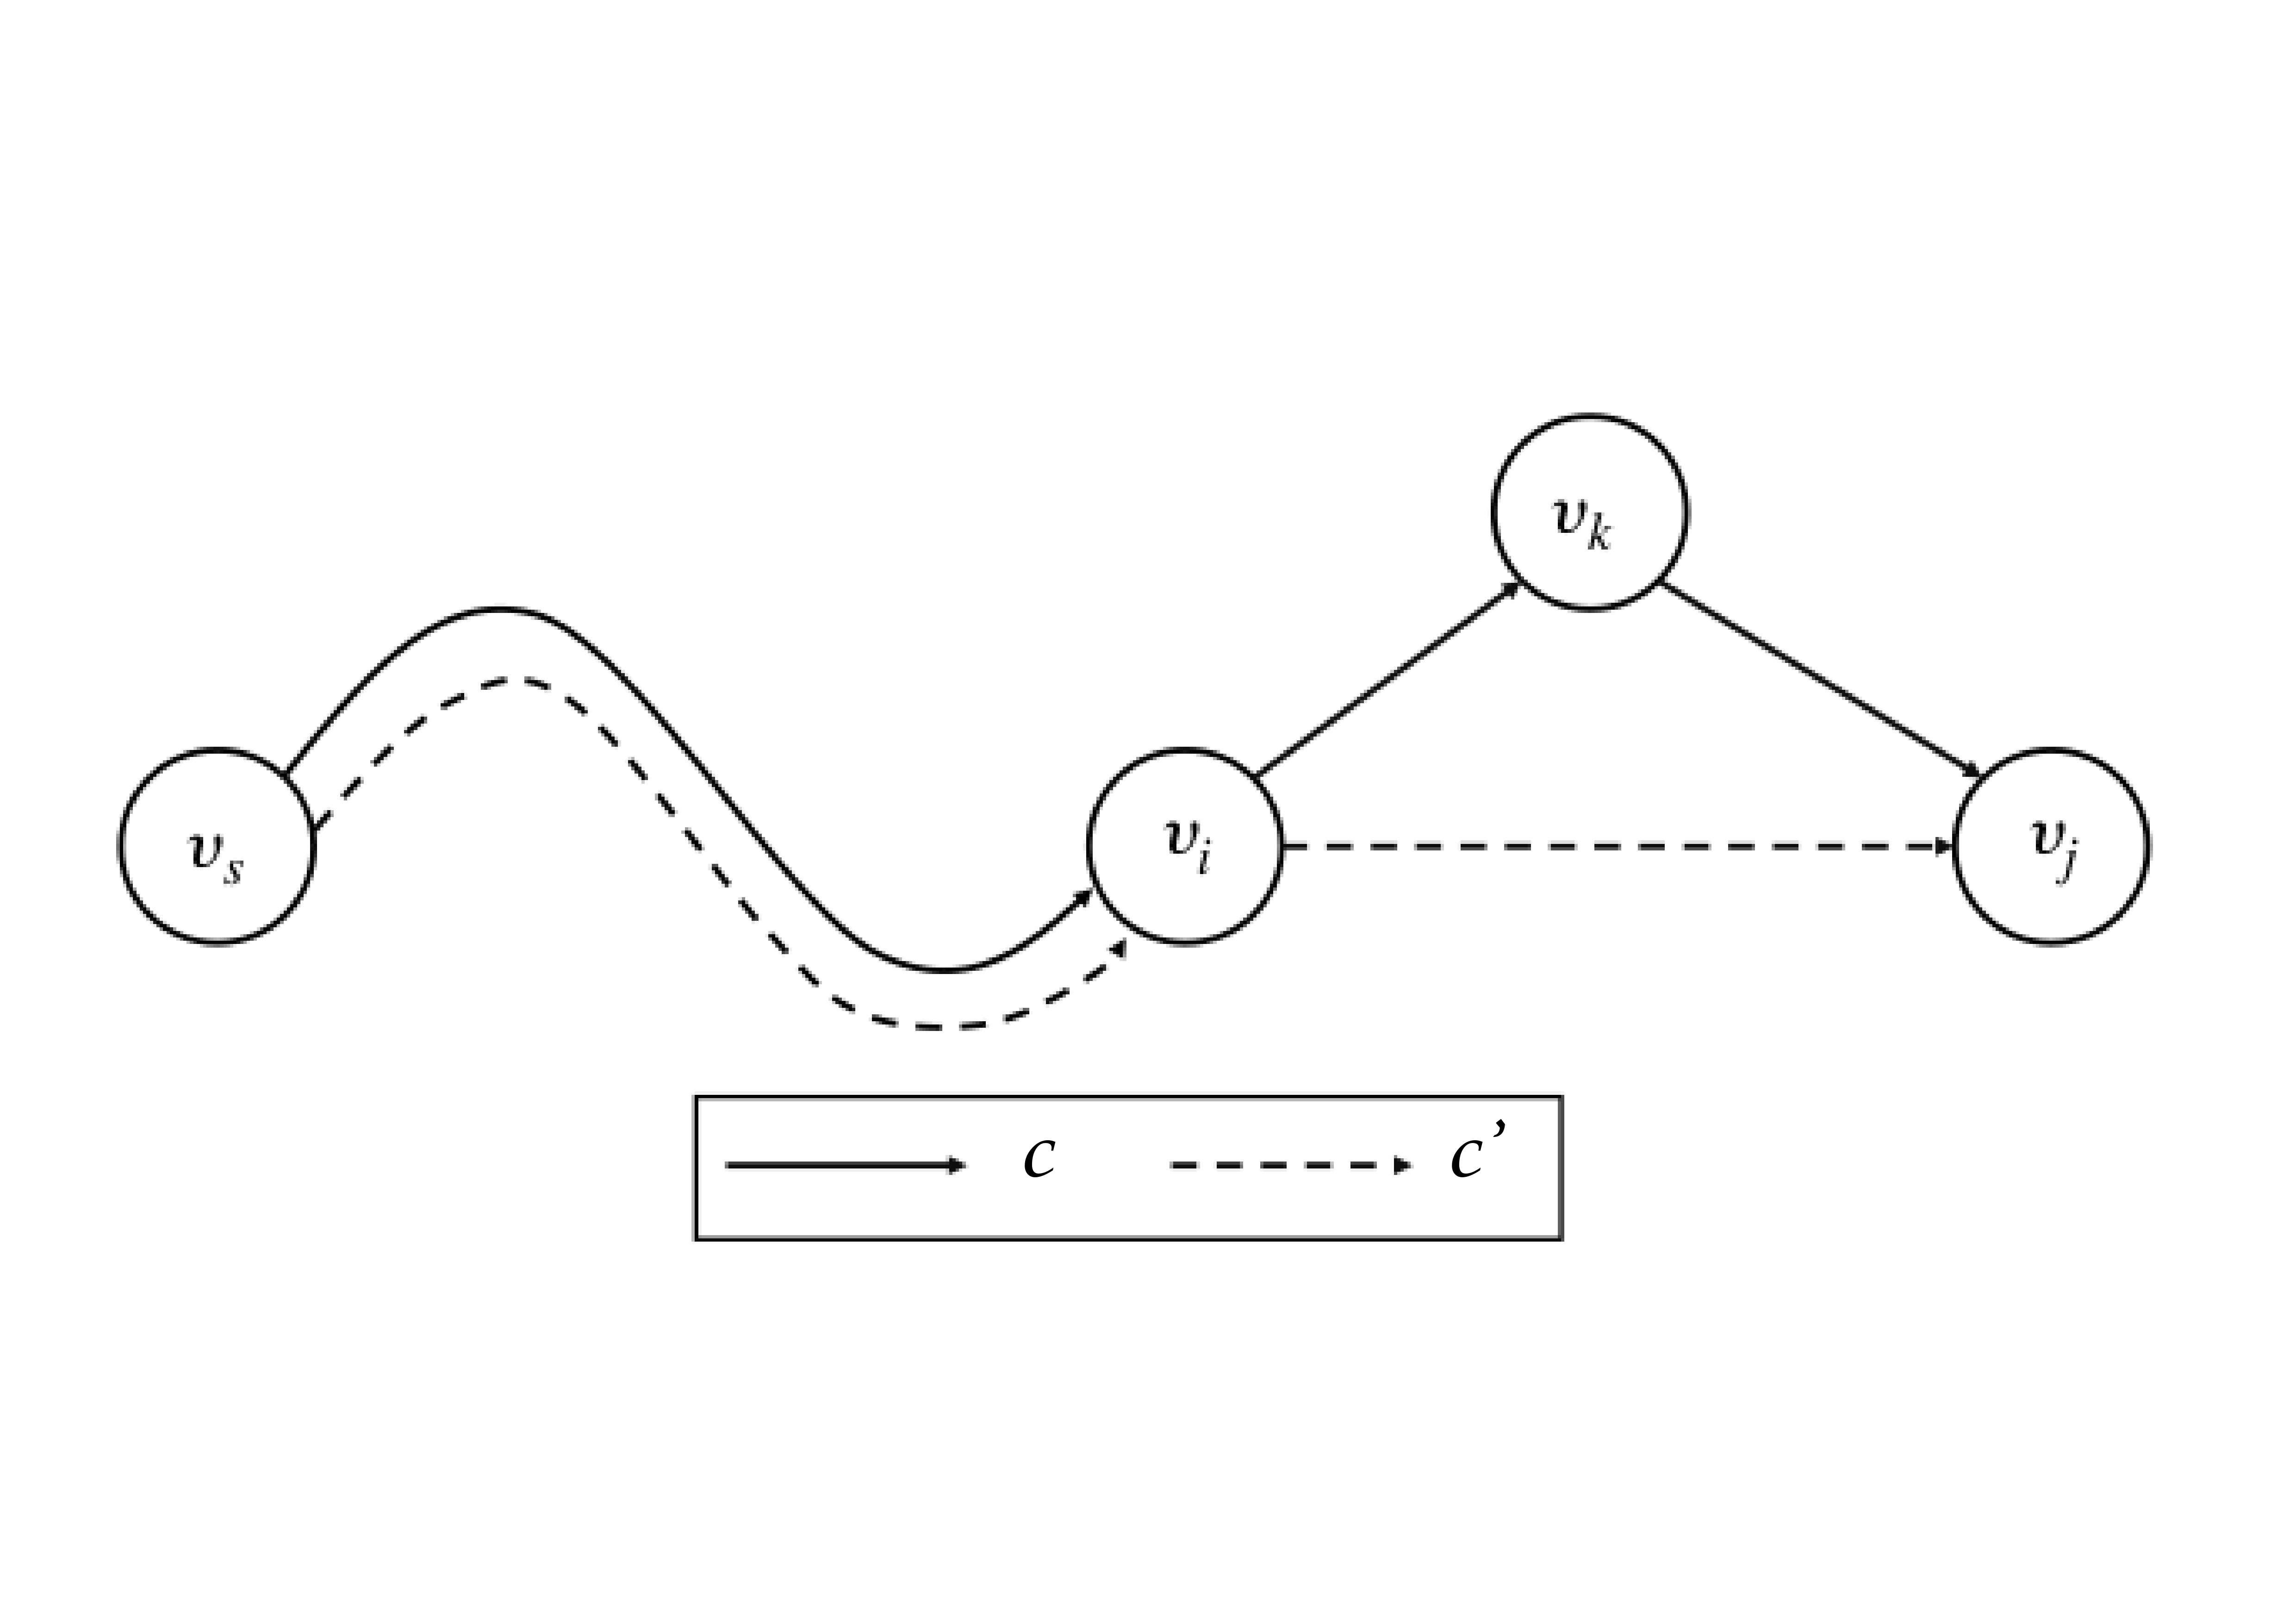
\includegraphics[width=0.5\textwidth]{img/rollback_pruning.jpg}
\caption{Representación gráfica de los caminos parciales}
\label{fig:rollback-pruning}
\centering
\end{figure}

El chequeo entonces se puede implementar en tiempo constante. Cada vez que agregamos un nodo $v_j$ a un camino parcial $C$ (con la regla de propagación de nodos), es fácil generar el correspondiente $C'$. Si para cada nodo $v_{\ell}$ de $C$ guardamos el precio acumulado, digamos $r_C(v_{\ell})$, entonces la condición
\begin{equation}
\label{eq:rollback-pruning-rule}
    r_C(v_i) + w_{v_i v_j} \leq r_C(v_k) + w_{v_k v_j}
\end{equation}
es suficiente para descartar a $C$. 

\subsubsection{Multirollback}

A esta estrategia de rollback inicial se le puede hacer una generalización. El camino $C'$ no necesariamente tiene que llegar hasta el antepenúltimo nodo de $C$ antes de ``saltar'' hasta $v_j$. En particular, si $C'$ es cualquier prefijo de $C$, que finaliza en el nodo $v_i$ (ahora este puede ser un nodo cualquiera de $C$) y luego ``salta'' a $v_j$, se siguen cumpliendo las condiciones $p(C') \subset p(C)$, $s(C') \subseteq s(C)$ y $q(C') \leq q(C)$. Entonces si se cumple \ref{eq:rollback-pruning-rule} también se puede descartar a $C$ y es bastante interesante que la ecuación que define la regla es exactamente la misma. 

El único truco aquí es que se modificaron las estructuras que se guardan en memoria asociadas a $v_i$ y ahora es necesario que cada camino parcial almacene los costos parciales de cada uno de sus prefijos.


\subsection{Modelo de Pricing con un algoritmo de Label Setting}
\label{section:pricing-labeling}

La formulación que proponemos en esta sección está basada en el algoritmo mono-direccional de programación dinámica propuesto por Righini \& Salani en \cite{righini-salani}. Esta publicación logró una gran repercusión en la comunidad científica que investiga el \problem{VRP} y merece la pena profundizarla.  Aquí los autores proponen una búsqueda bi-direccional acotada utilizando programación dinámica que bajo ciertas condiciones de simetría en el grafo puede resultar un enfoque eficiente para resolver \problem{ESPPRC}. En este trabajo nos limitamos a implementar la búsqueda mono-direccional del paper, la cual a su vez está basada en un trabajo de Feillet et al. \cite{feillet-et-al},y adaptarla a \problem{Star VRP} definido en \ref{star-pricing}.

Nos basamos en el algoritmo de Bellman-Ford para hallar caminos mínimos en un grafo pero con el agregado de las restricciones de recursos. Se asignan estados a cada vértice, donde cada estado representa un camino factible de $v_s$ hasta un vértice $i$. Cada estado contiene un vector de consumo de recursos y un costo. El objetivo del algoritmo es encontrar el estado asociado al vértice destino $v_e$ con menor costo.      
Una \emph{etiqueta} o \emph{label} es una tupla $L = (h_1, \dots, h_n, c, i)$ asociada al vértice $v_i$ que contiene la cantidad consumida $h_j$ de cada uno de los $n$ recursos y el costo reducido acumulado $c$ de un camino parcial factible que llega a $v_i$. El algoritmo \emph{extiende} recursivamente las etiquetas a medida que visita nuevos vértices, generando así nuevas etiquetas en las cuales el consumo de cada recurso y el precio deben ser actualizados, y en caso de superar alguna restricción de capacidad, la etiqueta descartada. Un algoritmo de estas características se conoce normalmente como \emph{algoritmo de label setting}, o en forma abreviada \emph{labeling}. Como regla general, estos se basan en un backtracking que extiende las etiquetas recursivamente de acuerdo a un conjunto de reglas de actualización hasta llegar a cubrir potencialmente la totalidad del espacio de búsqueda, y su eficiencia depende fuertemente de las reglas de poda que se definan.

En el caso particular de nuestro problema, tenemos el recurso $q$ que es la demanda acumulada, $p$ es el conjunto de nodos visitados y $s$ es el conjunto de clientes atendidos. Entonces las etiquetas son una $5-$tupla de la forma $L = (q, p, s, c, i)$. Indistintamente utilizamos la notación $q(L)$, $p(L)$, $s(L)$ y $c(L)$ para referirnos a estas variables. La etiqueta inicial es 

\begin{equation}
    L_0 = (0, \emptyset, \emptyset, -\lambda^{*}_0, v_s)
\end{equation}

Por la estructura del problema sería conveniente definir dos reglas de extensión. La primera se llama \emph{regla de extensión a nodos}, que atraviesa una arista del grafo para visitar un nuevo vértice $v_j$ pero no suma ningún cliente. Si $L' = (q', p', s', c', j)$ es la nueva etiqueta generada, entonces se actualiza así:

\begin{itemize}
    \item $p(L') \gets p(L) \cup \{v_j\}$
    \item $c(L') \gets c(L) + w_{ij}$
\end{itemize}

La segunda regla se llama \emph{regla de extensión a clientes}, cuyo camino parcial permanece en el vértice $v_i$ que se encontraba pero agrega un nuevo cliente $s$. Se hace:

\begin{itemize}
    \item $q(L') \gets q(L) + q_ s$
    \item $s(L') \gets s(L) \cup \{s\}$
    \item $c(L') \gets c(L) - \lambda^{*}_s$
\end{itemize}

Para descartar estados que son inalcanzables por cualquier extensión factible de $L_0$ alcanza con que se cumpla alguna de las siguientes condiciones:

\begin{itemize}
    \item $q(L') > Q$
    \item $v_j \in p(L)$
    \item $s \in s(L)$
\end{itemize}

Vamos a dar una definición clave:

\begin{definition}
\label{def:domination}
    (Relación de dominación).
    Una etiqueta $L$ \emph{domina a} $L'$, y se denota $L \preceq L'$, si ambas están asociadas al mismo vértice $v_i$ y se cumplen:
    \begin{enumerate}
        \item $q(L) \leq q(L')$
        \item $p(L) \subseteq p(L')$
        \item $s(L) \subseteq s(L')$
        \item $c(L) \leq c(L')$
    \end{enumerate}

Decimos que $L$ domina \emph{estrictamente} a $L'$ si alguna de las cuatro condiciones se cumple de manera estricta. Se denota $L \prec L'$
\end{definition}

Notemos que si $L \preceq L'$ y $L'$ es generada después de $L$, entonces $L'$ puede ser descartada. Intuitivamente, si dos caminos factibles llegan al mismo vértice, y el que está asociado a $L$ consumió menos recursos y conlleva un menor precio, entonces cualquier extensión posible de $L'$ puede ser dominada por una extensión equivalente de $L$. 

Al evitar extender una etiqueta no solamente estamos recortando un estado inalcanzable sino que estamos evitando toda una sección del espacio de búsqueda al cercenar las posibles extensiones de la misma. Esto motiva el uso de programación dinámica, ya que un almacenamiento apropiado para las etiquetas creadas nos permitiría verificar si esta es dominada por alguna anterior, y en ese caso inmediatamente descartarla.    

\subsubsection{Algoritmo}

En el Algoritmo \ref{al:label-setting} utilizamos la siguiente notación: $\Gamma$ es el conjunto de etiquetas que ya fueron visitadas, que tiene la capacidad de decidir si una nueva etiqueta es dominada por aquellas que ya están presentes, o si domina a alguna de ellas. Una cola de prioridad guarda las etiquetas que se han extendido recientemente para ser visitadas. $\Delta(v)$ es el conjunto de aristas salientes del vértice $v$. La función \texttt{isFeasible} simplemente chequea que una etiqueta corresponda a un camino válido en cuanto a las restricciones de recursos. Por otro lado, los procedimientos \texttt{extendWithNodeRule} y \texttt{extendWithCustomerRule} respectivamente crean una nueva etiqueta en base a las reglas ya explicadas.

\begin{algorithm}[H]
  \caption{Algoritmo de Label Setting}
  \label{al:label-setting}
  \begin{algorithmic}[1]
  	\Require Un grafo $G = (N, E)$ y las variables duales $\{\lambda^*_0, \dots, \lambda^*_{|S|}\}$.
  	\Ensure La ruta factible de menor precio $\mathscr{R}^{*}$.
        \State $\Gamma \gets \{L_0\}$
        \State $\texttt{queue} \gets \{L_0\}$
        \While{$\texttt{!queue.empty()}$}
            \State {Seleccionar y quitar $\ell = (q, p, s, c, v) \in \Gamma$}
            \If{$\neg \exists \ell' \in \Gamma : \ell' \preceq \bar{\ell}$}
                \ForEach{$s' \in \varrho^{-1}(v)$}
                    \State $\bar{\ell} \gets $ \texttt{extendWithCustomerRule} ($\ell$, $s'$)
                    \If{\texttt{isFeasible}($\bar{\ell}$) $\wedge$ $\neg \exists \ell' \in \Gamma : \ell' \preceq \bar{\ell}$}
                        \State $\Gamma \gets \Gamma \cup \{\bar{\ell}\}$
                        \State {\texttt{queue} $\gets$ \texttt{queue} $\cup \{\bar{\ell}\}$}
                    \EndIf
                \EndFor
                \ForEach{$v' \in \Delta(v)$}
                    \State $\bar{\ell} \gets $ \texttt{extendWithNodeRule} ($\ell$, $v'$)
                    \If{\texttt{isFeasible}($\bar{\ell}$) $\wedge$ $\neg \exists \ell' \in \Gamma : \ell' \preceq \bar{\ell}$}
                        \State $\Gamma \gets \Gamma \cup \{\bar{\ell}\}$
                        \State {\texttt{queue} $\gets$ \texttt{queue} $\cup \{\bar{\ell}\}$}
                    \EndIf
                \EndFor
            \EndIf
        \EndWhile
        \ForEach{$\ell = (q, p, s, c, v) \in \Gamma : v = v_e$}
            \If{$c < c(\mathscr{R}^{*})$}
                \State $\mathscr{R}^{*} \gets \ell$
            \EndIf
        \EndFor
        \Return $\mathscr{R}^{*}$
  \end{algorithmic}
\end{algorithm}


\subsubsection{Estructura de datos para almacenar etiquetas}

En la práctica, la elección de una estructura de datos apropiada para $\Gamma$ es clave para lograr una mejor complejidad computacional.

Para representar los conjuntos de clientes o nodos ($p(L)$ y $s(L)$) resulta conveniente utilizar un BitSet, cuya complejidad para verificar si un conjunto está incluido en otro es $\mathcal{O}(1)$. Esto permitiría realizar el chequeo de si una etiqueta domina a otra en $\mathcal{O}(1)$. 

Para $\Gamma$ usamos un diccionario que tiene como claves los BitSets que simbolizan $p(L)$ y como valores otro diccionario, cuyas claves son los valores de $s(L)$, en forma de BitSet, y cuyos valores son las etiquetas $L$. 

Bajo estos supuestos, la cantidad de etiquetas no puede ser infinita, aunque la cota no es muy alentadora. Se tiene que $|\Gamma| \leq 2^{|N|} \times 2^{|S|}$. La complejidad de búsqueda en esta estructura es proporcional a este valor, y eso da pie a la presentación de la próxima heurística.


\subsubsection{Heurística de Dominancia Relajada}
\label{subsubsection:segment-tree-heuristic}

Resolver el problema de pricing a optimalidad podría resultar demasiado costoso y en la práctica a menudo es innecesario. En rigor, tampoco es imprescindible hallar \emph{el menor} costo reducido en cada iteración del loop de generación de columnas, sino que basta con encontrar \emph{alguno(s)} que sean negativos, y agregar esas columnas a la base. Cuando se resuelve el \problem{RMP} a optimalidad, recién en la última iteración precisamos demostrar que ya no existen costos reducidos negativos. 

Una relación de dominación más débil que la definida en \ref{def:domination} resultaría en que el algoritmo \emph{domine de más} y por lo tanto descarte más etiquetas que lo necesario, lo cual es beneficioso para recortar el espacio de búsqueda pero se corre el riesgo de descartar un camino válido (el algoritmo dejaría de ser exacto). Es importante que se siga cumpliendo que todos los caminos generados sean válidos. A una relación que cumple estas características la llamamos dominación \emph{relajada}.

Una opción sería olvidarse de las condiciones de que $p(L) \subseteq p(L')$ y $s(L) \subseteq s(L')$ en la Definición \ref{def:domination}. En ese caso, la etiqueta de menor precio que visitó el nodo $v$ con demanda acumulada $q$ durante la ejecución del Algoritmo \ref{al:label-setting} dominaría a cualquier otra que pase por este nodo con esta demanda. Notemos que por esto la cantidad de etiquetas del almacenamiento estaría acotada por $|\Gamma| \leq |N| \times (Q+1)$, que es mucho más ajustada que en el caso general.

El almacenamiento de etiquetas $\Gamma$ pasa a ser una matriz de tamaño $\Gamma \in \mathbb{R}^{|N| \times (Q+1)}$ tal que $\Gamma_{iq}$ recuerda cuál es el camino factible de menor precio que visitó $v_i$ con demanda exactamente $q$. La relación de dominación se reduce a ver que existe otra entrada $\Gamma_{iq'}$ con $q' \leq q$ y precio menor. La implementación directa de este algoritmo implica recorrer todas las etiquetas con $q' \leq q$ para el mismo vértice y tiene una complejidad de inserción de $\mathcal{O}(1)$ y búsqueda de $\mathcal{O}(Q)$. Una estructura de datos apropiada nos permitiría mejorar esta complejidad.

En vez de emplear una matriz para representar a $\Gamma$, la estructura de datos que utilizamos consiste en un arreglo de estructuras independientes $\{\Gamma_1, \dots, \Gamma_{|N|}\}$, una por cada vértice de $|N|$. En vértice $v_i$, $\Gamma_i$ se representa como un \texttt{Segment Tree} que opera sobre un arreglo de longitud $Q + 1$ y que en cada posición $q$ guarda el mejor precio de un camino parcial factible que termina en $v_i$ y utiliza exactamente $q$ de demanda total. Esto es mejor que un arreglo común porque ahora consultar el menor precio entre todas las etiquetas $q' \leq q$ tiene una complejidad $\mathcal{O}(\log(Q))$. La complejidad de inserción de una etiqueta en el \texttt{Segment Tree} también es de $\mathcal{O}(\log(Q))$.

En la práctica, esta heurística no solamente acelera considerablemente la bús\-queda sino que también suele adivinar la ruta óptima global en la mayoría de los casos. Profundizaremos sobre esto en el capítulo de experimentación computacional.


\subsubsection{Eliminación de Simetría}

Un problema recurrente en el mundo de los problemas de optimización es el que refiere a distinguir soluciones factibles que son diferentes desde la semántica que se les da pero que tienen el mismo impacto en la función objetivo y por lo tanto seleccionar una de ellas es suficiente a efectos prácticos para hallar el óptimo. Descartar al resto de los miembros de la clase de equivalencia que queda definida bajo esta relación muchas veces es una tarea sencilla y basta con una pequeña perturbación del modelo original pero puede tener un impacto importante a nivel de performance. 

En el caso de \problem{Star ESPPRC}, si dos caminos parciales factibles tienen exactamente la misma demanda acumulada y el mismo costo reducido acumulado, nos resulta indistinto saber cuáles fueron los clientes atendidos para llegar a esos valores. Distinguir estas soluciones puede ser una buena idea para agregar casos de dominancia y por lo tanto recortar parte del espacio de búsqueda. Por ejemplo, supongamos que dos rutas tienen la misma trayectoria y atendieron al mismo conjunto de clientes pero en distinto orden. Realmente no tiene sentido que el algoritmo sacrifique tiempo valioso en considerar ambas posibilidades cuando a efectos prácticos son indistinguibles. 

Una idea clásica es la modificación de la función objetivo de manera que dos soluciones anteriormente equivalentes ahora tengan un impacto levemente distinto, lo suficiente para recortar alguna de ellas pero no tan grande para que otra solución no equivalente y subóptima pueda tener un mejor valor. Siguiendo estas líneas, proponemos agregar un pequeño costo $\tilde{w}_s$ asociado a atender a un cliente $s$, de manera que la función objetivo quede alterada. El \emph{precio modificado} de una ruta factible $r$ se define como:

\begin{equation}
    \tilde{c}_r = \sum_{(i, j) \in E}{w_{ij}} - \lambda^*_0 - \sum_{s \in \tilde{S}_r}{\lambda^*_s} + \sum_{s \in \tilde{S}_r}{\tilde{w}_s}
\end{equation}

Nos gustaría que si $r_1$ tiene menor costo reducido que $r_2$, entonces el precio modificado preserve esta relación, aunque el recíproco no es cierto. Esto es, $\bar{c}_{r_1} < \bar{c}_{r_2} \Rightarrow \tilde{c}_{r_1} < \tilde{c}_{r_2}$. Para eso se tiene que cumplir:

\begin{equation}
    \sum_{s \in \tilde{S}_r}{\tilde{w}_s} < \varepsilon \quad \forall \tilde{S}_r \subseteq S
\end{equation}

Donde $\varepsilon$ debe ser tal que $\bar{c}_{r_1} - \bar{c}_{r_2} > \varepsilon$ para todos $r_1, r_2 \in \Omega$ tales que $\bar{c}_{r_1} - \bar{c}_{r_2} > 0$. En la práctica es suficiente tomar $\varepsilon = 1$.

En el algoritmo se implementó de la siguiente manera: supongamos que un cliente $s$ es atendido desde un nodo $v$ (por supuesto, $v \in \varrho(s)$), luego basta $\tilde{w}_s = \alpha w_{vs}$, donde
\begin{equation}
    \alpha = \frac{\varepsilon}{\sum_{(i,j) \in E}{w_{ij}}}
\end{equation}
y de esta manera se cumple
\begin{equation}
    \sum_{s \in \tilde{S}_r}{\tilde{w}_s} = 
    \sum_{(v, s) \in r}{\alpha w_{vs}} = 
    \varepsilon \frac{\sum_{(v, s) \in r}{w_{vs}}}{\sum_{(i,j) \in E}{w_{ij}}} < 
    \varepsilon
\end{equation}

Coloquialmente, podemos pensar que el problema de elegir el camino en sí y el problema de elegir los clientes con un camino dado son problemas independientes, pero que al tener que investigar todas las combinaciones de ambos se produce una explosión de casos que sin dudas agrega una dificultad adicional. No en todas las variantes del problema de ruteo de vehículos se ve este fenómeno, y por lo tanto, \problem{Star VRP} pareciera ser una particularmente dura. 

\section{2-Step Column Generation}
\label{section:2-step-cg}

Si uno decidiera listar las rutas que hay en la base y las que se van agregando en cada iteración, una breve inspección visual advierte un fenómeno reiterado. El algoritmo de generación de columnas es bastante rápido para encontrar buenas trayectorias (circuitos que pasan por el depósito) pero demora muchas iteraciones en encontrar la combinación exacta de clientes que minimiza la función objetivo.  

En instancias grandes, una sola iteración de generar columnas puede ser com\-putacionalmente exhaustiva. Si encontrásemos un mecanismo para asignar los clientes restringido al listado histórico de rutas halladas, es probable que podamos ahorrar varias corridas del algoritmo de pricing. Además, podemos combinar esta idea con una heurística para calcular los caminos de costo reducido negativo, aún así es necesario disponer de un mecanismo para terminar la ejecución, ya que actualmente el algoritmo termina cuando no hay más columnas por agregar.

Por este motivo proponemos un algoritmo de generación de columnas en dos pasos: el primer paso es el problema de pricing que aporta una lista de trayectorias válidas a la base y en una segunda fase se corre otro algoritmo que reordena los clientes, mejorando la solución del pricing.

Una implementación razonable podría ser la siguiente. Tomemos el acumulado de rutas factibles que el algoritmo ya encontró y olvidemos los clientes que visita cada una. Ahora el desafío consiste en asignar el conjunto de clientes $S$ a un subconjunto de rutas de tamaño a lo sumo $|K|$, de manera que se respeten las capacidades de los vehículos y que cada cliente sea atendido desde una parada válida. Con estas restricciones nos gustaría encontrar el subconjunto menos costoso que las satisfaga. Obsérvese que este problema es muy similar al problema de \emph{factibilidad} propuesto en \ref{feasibility-problem}. Lamentablemente esta idea se descartó porque si bien implementar un modelo de programación lineal entera que resuelva este problema es una tarea directa, no cumple con su propósito original si es más lento que correr el algoritmo de pricing. 

Entonces incurriremos una vez más en el enigmático mundo de las heurísticas. Nos basamos en la siguiente idea: \problem{Star VRP} nos permite que varios vehículos tengan la misma ruta, ya que podrían atender distintos conjuntos de clientes, entonces tiene sentido reutilizar las rutas más baratas y con ellas cubrir todo lo que sea posible. 

Utilizamos la siguiente notación: $\tilde{\Omega}$ es el conjunto de rutas descubiertas hasta el momento por el algoritmo de generación de columnas. Una ruta $r$ (cuya trayectoria es el camino $C_r$) tiene un conjunto de \emph{clientes potenciales}, que notamos $\nu(r)$, y corresponde a todos los clientes que pueden ser atendidos desde algún nodo de $C_r$, ignorando las restricciones de capacidad. Esto es:

\begin{equation}
    \nu(r) = \{s \in S : \exists v \in C_r \wedge v \in \varrho(s)\} = \bigcup_{v \in C_r}{\varrho^{-1}(v)}
\end{equation}

El siguiente algoritmo tiene como objetivo encontrar algunas rutas factibles que no están en $\tilde{\Omega}$ pero que son rutas ``razonables'', para poder agregarlas a este conjunto antes de la próxima iteración. Llamamos $\Omega^{*}$ al conjunto de rutas factibles que se descubren con este algoritmo. Vale que $\Omega^{*} \subset \Omega$ y $\Omega^{*} \cap \tilde{\Omega} = \emptyset$.

\begin{algorithm}[H]
  \caption{Heurística para mejorar asignación de clientes a rutas}
  \label{al:2-step-cg-main}
  \begin{algorithmic}[1]
  	\Require $\tilde{\Omega}$ un conjunto de rutas factibles.
  	\Ensure $\Omega^{*}$ una asignación de rutas a vehículos. 
        \State $\Omega^{*} \gets \emptyset$
        \ForEach {$s \in S$}
            \If {$s$ no es atendido por $\Omega^{*}$}
                \State Sea $r$ la ruta de menor costo de $\tilde{\Omega}$ que atiende a $s$.
                \State Calcular $\nu(r)$.
                \State Calcular $\mathscr{P}$, una partición factible minimal de $\nu(r)$, con el Algoritmo \ref{al:feasible_minimal_partition_algorithm}
                \State $m \gets |\mathscr{P}|$.
                \State Crear un conjunto de rutas $\{r_1, \dots, r_m\}$, cuya trayectoria es una copia de $r$, pero cada una atiende a un conjunto de clientes distinto de $\mathscr{P}$.
                \State $\Omega^{*} \gets \Omega^{*} \cup \{r_1, \dots, r_m\}$.
            \EndIf
        \EndFor
	\Return $\Omega^{*}$
  \end{algorithmic}
\end{algorithm}

Para mejorar un poco esta solución se puede reforzar con otra heurística. Se dice que un par de rutas $r_1, r_2 \in \Omega^{*}$ puede ser \emph{mejorado} por una única ruta $r^{*} \in \Omega$ si esta ultima es menos costosa que la suma de $r_1$ y $r_2$ y los clientes atendidos por $r_1$ y $r_2$ pueden atenderse desde desde $r^{*}$ sin violar las restricciones de capacidad.

Un algoritmo ``burbuja'' chequea todos los pares de rutas hasta encontrar uno que pueda ser \emph{mejorado}. El pseudocódigo luce así:

\begin{algorithm}[H]
  \caption{Algoritmo burbuja para \emph{mejorar} rutas factibles}
  \label{al:bubble-algorithm}
  \begin{algorithmic}[1]
  	\Require $\Omega^{*}$ una asignación de rutas a vehículos. 
  	\Ensure $\Omega^{**}$ una asignación \emph{mejorada} de rutas a vehículos. 
        \While {$\exists r_1, r_2 \in \Omega^{*}, r_3 \in \Omega : r_3$ mejora a $\{r_1, r_2\}$}
            \State $\Omega^{*} \gets \Omega^{*} \cup \{r_3\} \setminus \{r_1, r_2\}$
        \EndWhile
	\Return $\Omega^{*}$
  \end{algorithmic}
\end{algorithm}

En la Sección \ref{section:2-step-cg-testing} nos encargamos de probar cuánto mejora el rendimiento general del algoritmo de generación de columnas con esta heurística.

\section{Terminación temprana}
\label{section:finish-early}

A menudo sucede que no interesa resolver la relajación lineal del \problem{RMP} a optimalidad y para eso vimos algoritmos aproximados. Uno de los problemas existenciales que aparecen en un modelo de generación de columnas es la definición de la condición de terminación, que por lo general suele implicar agotar el problema de pricing hasta que no haya nuevas columnas por agregar. Sería ideal encontrar una condición para terminar el loop de manera adelantada mientras nos asegure que la solución no esté demasiado lejos del óptimo.

Cuando uno examina la dinámica con la cual va convergiendo la solución incumbente del \problem{RMP} hacia el óptimo, notamos ciertas regularidades. En la siguiente figura se aprecia un ejemplo clásico de convergencia en generación de columnas. 

\begin{figure}[H]
\centering
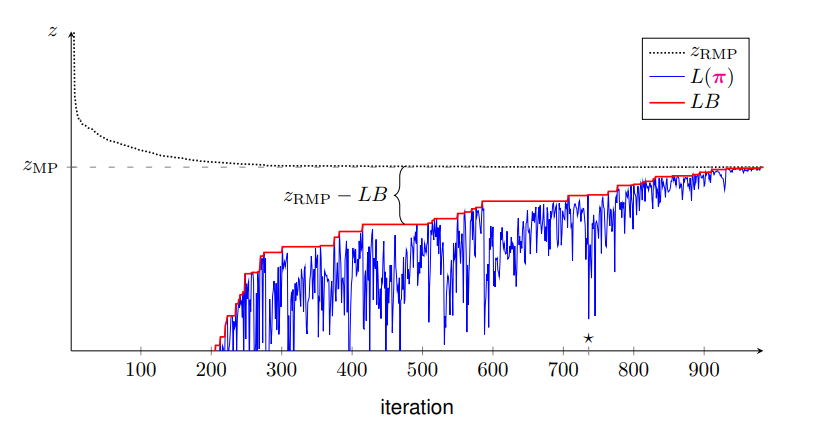
\includegraphics[width=0.7\textwidth]{img/Screenshot from 2023-10-11 00-03-23.png}
\caption{Convergencia de la solución incumbente y la cota inferior, en un ejemplo de Lübbecke. (Fuente: \cite{co-at-work-luebbecke})}
\label{fig:bound-convergence}
\centering
\end{figure}

En un problema de minimización, la solución de cada iteración es monótonamente decreciente, ya que en cada paso agregamos variables a la base que solamente pueden mejorar la solución. Esta solución incumbente es una cota superior del óptimo, por lo que si se pueda establecer una cota inferior, entonces tenemos un techo para la brecha entre el óptimo incumbente y el óptimo real. Por lo tanto, cuando el gap sea menor que un valor aceptable, se puede detener el bucle.

Llamemos $z_{RMP}$ al óptimo incumbente, y $z_{MP}$ al óptimo global. En \cite{desrosiers2005primer} Desrosiers \& Lübbecke proponen una cota ajustada que soluciona este problema. Si tenemos un valor real $\kappa$ que cumple $\sum_{\theta_r \in \Omega} \leq \kappa$ y $\bar{c}^{*}$ es el menor costo reducido, entonces vale
\begin{equation}
    z_{RMP} + \kappa \bar{c}^{*} \leq z_{MP} \leq z_{RMP}
\end{equation}

En la Figura \ref{fig:bound-convergence} se utiliza $L(\pi) = z_{RMP} + \kappa \bar{c}^{*}$ y $LB$ es el máximo valor de $L(\pi)$ hasta el momento.

Notemos que por \ref{eq:master2}, podemos tomar $\kappa = |K|$. Por lo tanto la condición de parada temprana es la siguiente:
\begin{equation}
     \frac{|(z_{RMP} + |K| \bar{c}^{*}) - z_{RMP}|}{z_{RMP}} = \frac{-|K| \bar{c}^{*}}{z_{RMP}}  < THRESH
\end{equation}

La única desventaja que tiene este método es que para conseguir el menor costo reducido sigue siendo necesario resolver el problema de pricing a optimalidad. Esta aclaración es importante ya que no vamos a poder combinar esta heurística con algoritmos que resuelvan el pricing de manera aproximada.

En la sección de experimentación hablaremos sobre los parámetros reales con los que configuramos este algoritmo. Resultaría razonable que el umbral esté en el orden del $1\%$.
